\chapter{稳定化}\label{ch:stability}

数学中的许多问题都归结为按某种等价关系对特定对象分类。通常无法对所有对象完成分类，也无法为分类空间赋予良好的几何结构。应对这类问题的一种思路，是对对象空间施加额外条件，使分类问题的性质更好；这类条件称为稳定性条件。本章讨论表示论中两种主要稳定性条件：用于构造代数表示模空间的 King 稳定性\bookcite{138} 和用于研究导出范畴结构的 Bridgeland 稳定性\bookcite{39}。我们将在曲面的 Fukaya 范畴、gentle 代数和 Jacobi 代数中讨论这些稳定性条件，研究它们之间的关系，并给出几何解释。

\section{格罗滕迪克群}\label{sec:grothendieck-group}

格罗滕迪克群\index{geluotengdikequn@格罗滕迪克群|hyperpage}\bookcite{99}是分类对象最粗略的方法之一。本节定义 $A_\infty$ 范畴的格罗滕迪克群，并考察拓扑 Fukaya 范畴的情形。关于格罗滕迪克群及更一般的 $K$ 理论，参见 Weibel 的著作\bookcite{254}。分次曲面的格罗滕迪克群构造见\bookcite{115}；Abouzaid 在\bookcite{4}中对闭曲面的 Fukaya 范畴作了类似计算。
\takeaway{格罗滕迪克群 $K_0A^{\bullet}$ 由对象符号模去拟同构、平移与锥关系生成；对分次曲面有 $K_0\mathrm{topFuk}^{\bullet}(\vec S,M)\cong H_1(\vec S,M)$，Euler 型给出双线性形式，其核给出数值格罗滕迪克群。}

\begin{definition}{格罗滕迪克群}{grothendieck-group}
设 $A^{\bullet}$ 是对平移和锥封闭的 $A_\infty$ 范畴。格罗滕迪克群 $K_0A^{\bullet}$ 是由符号 $[X]$（其中 $X$ 是 $A^{\bullet}$ 的对象）生成的自由阿贝尔群，再对以下关系取商所得的群：
\begin{itemize}
  \item 若 $X,Y$ 拟同构，则 $[X]-[Y]=0$；
  \item $[X]+[X[1]]=0$；
  \item 若 $f\colon X\to Y$ 是次数为 $1$ 的态射，则 $[X]+[Y]-[\operatorname{Cone}(f)]=0$。
\end{itemize}
若 $A^{\bullet}$ 对平移和锥不封闭，则记 $K_0A^{\bullet}:=K_0\mathrm{Tw}A^{\bullet}$。最后一条关系蕴含：对扭曲复形 $(M,\delta)$，有
\[
  [(M,\delta)]=[M].
\]
\end{definition}

\begin{example}[向量空间与群表示]
$D\mathrm{vect}^{\bullet}$ 的格罗滕迪克群是 $\mathbb Z$，因为每个对象都是一维向量空间平移的直和。类似地，若 $G$ 是有限群，则
\[
  K_0D\mathrm{mod}^{\bullet}\mathbb CG\cong\mathbb Z^k,
\]
其中 $k$ 是 $G$ 的不可约表示个数。
\end{example}

\begin{example}[多项式环的模]
考虑 $R=\mathbb C[X]$。每个有限生成模都有长度不超过 $1$ 的自由分解，故在格罗滕迪克群中其类由 $[R]$ 与 $[S^\lambda]$ 生成。这里 $S^\lambda$ 是映射
\[
  m_{X-\lambda}\colon R\longrightarrow R,\qquad
  r\longmapsto(X-\lambda)r
\]
的锥，因此在格罗滕迪克群中
\[
  [S^\lambda]=[R]-[R]=0.
\]
所以 $K_0\mathrm{Mod}^{\bullet}R\cong\mathbb Z$，它测量模无挠部分的秩。另一方面，若只考虑有限维模的导出范畴 $D\mathrm{mod}^{\bullet}R$，上述约化无法进行，故 $K_0\mathrm{mod}^{\bullet}R$ 由无穷多个生成元 $[S^\lambda]$ 自由生成。
\end{example}

\begin{theorem}{无环箭图的格罗滕迪克群}{acyclic-quiver-grothendieck}
设 $Q$ 是没有有向环的箭图，则
\[
  K_0D\mathrm{Mod}^{\bullet}Q\cong\mathbb Z^{Q_0}.
\]
\end{theorem}
\begin{proof}[证明思路]
由于 $Q$ 没有有向环，顶点简单模生成有限维模，因此有满射
\[
  \phi\colon\mathbb Z^{Q_0}\longrightarrow K_0D\mathrm{mod}^{\bullet}Q.
\]
另一方面，对模复形 $M^{\bullet}$，令
\[
  \alpha(M^{\bullet}):=\sum_i(-1)^i\underline{\dim}_{\mathrm{vect}} H^i(M^{\bullet}).
\]
对次数为 $1$ 的态射 $f\colon M\to N$，有
\[
  \alpha(M[1]^{\bullet})=-\alpha(M^{\bullet}),\qquad
  \alpha\bigl(\operatorname{Cone}(f\colon M\to N)\bigr)
  =\alpha(M)+\alpha(N).
\]
故得到满射 $\alpha\colon K_0D\mathrm{mod}^{\bullet}Q\to\mathbb Z^{Q_0}$。这两个映射互为逆映射。
\hfill$\square$
\end{proof}

设 $(\vec S,M)$ 是分次带标记曲面，$A$ 是将它剖分的弧系。由于这些弧生成拓扑 Fukaya 范畴，得到满射
\[
  \mathbb Z A\longrightarrow K_0\mathrm{topFuk}^{\bullet}(\vec S,M).
\]
若 $a_1,\ldots,a_k$ 围成一个多边形，内部角为 $\alpha_i\colon a_i\to a_{i+1}$，则在拓扑 Fukaya 范畴中有同构
\[
  \left(a_1[i_1]\oplus\cdots\oplus a_{k-1}[i_{k-1}],
  \alpha_1+\cdots+\alpha_{k-2}\right)
  \cong a_k[i_k-1],
\]
其中各平移 $i_j$ 的选取使所有 $\alpha_j\colon a_j[i_j]\to a_{j+1}[i_{j+1}]$ 都是次数为 $1$ 的态射。在格罗滕迪克群中，这给出关系
\[
  (-1)^{i_1}[a_1]+\cdots+(-1)^{i_k}[a_k]=0.
\]
令 $G_A$ 为由 $a_i$ 生成、并满足上述多边形关系的阿贝尔群。若分次来自向量场，则它与 $\mathbb Z_2$ 分次相容，可以把弧理解为定向线段；此时关系就是说，围成多边形边界的弧之和为零。弧可视为相对于 $M$ 的 $S$ 中的一个循环，因此 $G_A$ 可识别为相对第一同调。若分次并非来自向量场，仍可作类似解释：此时 $G_A$ 是以 $S$ 上某个层为系数、相对于 $M$ 的同调。细节见\bookcite{115}。本书只需作如下定义：
\[
  H_1(\vec S,M):=G_A.
\]
容易验证，该定义不依赖弧系 $A$ 的选择。

\begin{theorem}{分次曲面的格罗滕迪克群}{graded-surface-grothendieck}
\textnormal{（Haiden--Katzarkov--Kontsevich）}有
\[
  K_0\mathrm{topFuk}^{\bullet}(\vec S,M)
  \cong H_1(\vec S,M).
\]
\end{theorem}
\begin{proof}[证明思路]
若 $(S,M)$ 没有内部标记点，可找到一组不围成闭多边形的弧系。此时 $G_A$ 中没有关系，且 $\mathrm{Gtl}A$ 是没有有向环、也没有高阶乘积的带分次路径代数，可应用前一定理。一般情形下，可把 $\mathrm{topFuk}^{\bullet}(\vec S,M)$ 看作 $\mathrm{topFuk}^{\bullet}(\vec S',M')$ 的局部化，其中 $(\vec S',M')$ 没有内部标记点。利用\bookcite{99}中的结果，可通过正合列关联两者的格罗滕迪克群。更多细节见\bookcite{115}。
\hfill$\square$
\end{proof}

若 $A^{\bullet}$ 是 proper $A_\infty$ 范畴，即所有 Hom 空间的同调都有限维，则可在其格罗滕迪克群上定义双线性形式。

\begin{definition}{Euler 型}{euler-pairing}
$A^{\bullet}$ 的 Euler 型\index{eulerxing@Euler 型|hyperpage}是映射
\[
  \langle-,-\rangle\colon K_0A^{\bullet}\times K_0A^{\bullet}\longrightarrow\mathbb Z,
  \qquad ([X],[Y])\longmapsto\sum_i(-1)^i\dim A^i(X,Y).
\]
\end{definition}
% [Tutor Note: 定义中 $A^{i}(X,Y)$ 指分次 $\mathrm{Hom}$ 复形的第 $i$ 次部分，$\dim$ 是它的普通维数；交错和保证 $\langle X[1],Y\rangle=-\langle X,Y\rangle$，与格罗滕迪克群中 $[X[1]]=-[X]$ 相容。核对符号时可用这条恒等式自检。]

\begin{example}[无环箭图的 Euler 型]
设 $Q$ 没有有向环，$S_1,S_2$ 是两个有限维表示。由于不存在更高阶 Ext，双线性形式为
\[
  \langle S_1,S_2\rangle
  =\dim\operatorname{Hom}_{\mathbb CQ}(S_1,S_2)
  -\dim\operatorname{Ext}^1_{\mathbb CQ}(S_1,S_2).
\]
$S_i$ 在格罗滕迪克群中的类只依赖其维数向量 $\alpha_i$：
\[
  \langle S_1,S_2\rangle
  =\sum_{v\in Q_0}\alpha_1(v)\alpha_2(v)
  -\sum_{a\in Q_1}\alpha_1(t(a))\alpha_2(h(a)).
\]
\end{example}

\begin{example}[带对象的交数]
设 $(S,M)$ 是没有内部标记点的带标记曲面。若 $B_1=B(L_1,\lambda_1)$、$B_2=B(L_2,\lambda_2)$ 是两个带对象，则 $K_0\mathrm{topFuk}^{\pm}(S,M)$ 上的配对对应于两条曲线的交数：
\begin{figure}[H]\centering
  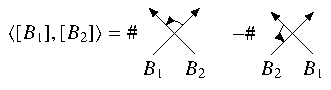
\includegraphics[width=0.30\textwidth]{figures/Fig_225_PDF327_Book315.pdf}
  \caption{带对象的交点及其符号（原书 p.315）}\label{fig:band-euler-intersection}
\end{figure}
在此情形下，带对象之间的配对是反对称的；若涉及弦对象，则一般不反对称。
\end{example}

很多情况下，格罗滕迪克群不是有限生成的，但可借助 Euler 型将其映到一个较小的群。

\begin{definition}{数值平凡元与数值格罗滕迪克群}{numerical-grothendieck-group}
若 $x\in K_0A^{\bullet}$ 满足对任意 $y\in K_0A^{\bullet}$ 都有 $\langle x,y\rangle=0$，则称 $x$（左）数值平凡。（左）数值格罗滕迪克群是格罗滕迪克群对数值平凡子群取商所得的群。
\end{definition}

\begin{note}[右数值格罗滕迪克群]
也可以定义右数值格罗滕迪克群；一般而言，它可能不同于左数值格罗滕迪克群。然而，若 $A_\infty$ 范畴光滑且 proper，则左右数值格罗滕迪克群相同，并且是有限生成群。证明见\bookcite{240}。
\end{note}

\begin{example}[带对象的数值类]
设 $(\vec S,M)$ 是分次带标记曲面，考虑由带对象生成的子范畴
\[
  \mathrm{Bands}^{\bullet}\subset\mathrm{topFuk}^{\bullet}(\vec S,M).
\]
一般而言，$K_0\mathrm{Bands}^{\bullet}$ 不是有限生成的。若两个带对象 $B_1,B_2$ 的底层简单曲线相同，它们在 $K_0\mathrm{Bands}^{\bullet}$ 中通常仍给出不同元素，但在数值格罗滕迪克群中代表同一元素，因为
\[
  \langle[B_1]-[B_2],-\rangle=0.
\]
\end{example}

\section{King 稳定性与裤子分解}\label{sec:king-stability-pants}

若 $Q$ 是箭图，$A=\mathbb CQ/I$ 是带关系的路径代数，可以通过构造半稳定表示的模空间来尝试分类表示。回忆第\ref{subsec:moduli-spaces}节中，我们曾利用维数向量 $\alpha\colon Q_0\to\mathbb N$ 和向量 $\theta\colon Q_0\to\mathbb Z$ 构造空间
\[
  M_\theta(A,\alpha)=\operatorname{Proj}(R_\theta),
\]
其中
\[
  R_\theta:=\bigoplus_{i=0}^{\infty}
  \left\{f\in\mathcal O(\operatorname{Rep}(A,\alpha))\ \middle|\
  \forall g\in\mathrm{GL}_\alpha,\quad
  g\cdot f=\left(\prod_{v\in Q_0}\det(g_v)^{\theta_v}\right)f\right\}.
\]
若 $\theta\cdot\alpha\ne0$，则该空间为空。其点对应于 $\theta$ 稳定表示的直和的同构类；所谓 $\theta$ 稳定，是指表示中不存在真子表示，其维数向量 $\beta$ 满足 $\beta\cdot\theta\le0$。这种稳定性常称为 King 稳定性，因为 Alistair King 在\bookcite{138}中对此作了深入研究。
\takeaway{King 稳定性用维数向量 $\alpha$ 与参数 $\theta$ 构造半稳定表示的模空间；环面二聚体的稳定完美匹配给出匹配多边形的三角剖分，Ishii--Ueda 定理把通有 $\theta$ 的模空间实现为环簇消解，其镜像由裤子曲面沿对偶图粘合而成。}
% [Tutor Note: 条件 $\beta\cdot\theta\le0$ 的方向与 $\theta$ 的选取绑定：把 $\theta$ 换成 $-\theta$ 就把 $\theta$ 稳定换成反稳定。另外模空间非空要求 $\theta\cdot\alpha=0$，所以 $\theta$ 只在 $\alpha$ 的正交补中取值；核对 King 稳定性时先检查这两个约定。]

现在用 King 稳定性研究带标记曲面的镜像对称。第九章中我们看到，构造镜像的一种方法是采用二聚体模型 $Q$ 及其 Jacobi 代数。若环面上的二聚体模型锯齿一致，则 $(\mathrm{Jac}(Q),\ell)$ 可视为非交换 Landau--Ginzburg 模型，并且镜像于对偶二聚体。

依照\bookcite{42,125,35}，考虑其 Jacobi 代数 $\mathrm{Jac}=\mathrm{Jac}(Q)$、固定维数向量 $\alpha\colon Q_0\to\mathbb N$（将每个顶点映为 $1$）的表示空间。表示空间 $\operatorname{Rep}(\mathrm{Jac}(Q),\alpha)$ 是仿射概形，其坐标环为
\[
  \mathbb C[\operatorname{Rep}(\mathrm{Jac}(Q),\alpha)]
  =\mathbb C[x_a\mid a\in Q_1]
  \Big/\left\langle\prod_{b\in l_a}x_b-\prod_{b\in r_a}x_b\ \middle|\ a\in Q_1\right\rangle.
\]
每条箭 $a$ 对应一个变量 $x_a$。若表示 $\rho$ 对每条箭都取非零值 $\rho(a)=x_a\ne0$，则称 $\rho$ 为环面表示。环面表示构成表示空间中的开集，其闭包是一个分支
\[
  \operatorname{Trep}(\mathrm{Jac}(Q),\alpha)\subset\operatorname{Rep}(\mathrm{Jac}(Q),\alpha),
\]
称为环面表示概形。给定稳定条件 $\theta$，可考虑环面表示的 $\theta$ 稳定模空间
\[
  M^t_\theta(\mathrm J,\alpha)\subset M_\theta(\mathrm J,\alpha).
\]
若 $\theta$ 通有，即对所有 $0<\beta<\alpha$ 都有 $\theta\cdot\beta\ne0$，则这是一个光滑环簇。Ishii 和 Ueda 研究了此环簇在通有 $\theta$ 下的结构\bookcite{125}。为概述其结果，先作如下定义。

\begin{definition}{完美匹配、多边形与余支撑}{perfect-matching-polygon-cosupport}
设 $Q$ 是环面上的一致二聚体模型，$X,Y\in\mathrm{Jac}\,Q$ 是张成环面同调的两个循环路径。
\begin{itemize}
  \item 完美匹配\index{wanmeipipei@完美匹配|hyperpage} $P$ 是箭的集合：二聚体的每个面 $c\in Q_2$ 都恰好含有一条属于 $P$ 的箭。给 $P$ 赋予一个分次 $\deg_P$，其中 $a\in P$ 时 $\deg_P(a)=1$，否则 $\deg_P(a)=0$。
  \item $P$ 对应的格点为 $m_P=(\deg_P X,\deg_P Y)$。
  \item 匹配多边形\index{pipeiduobianxing@匹配多边形|hyperpage}是所有 $m_P$ 的凸包。
  \item 表示 $\rho$ 的余支撑是取值为零的箭集 $\{a\mid\rho(a)=0\}$。
  \item 若完美匹配集 $\{P_1,\ldots,P_k\}$ 的并是某个 $\theta$ 稳定表示的余支撑\index{biaoshideyuzhicheng@表示的余支撑|hyperpage}，则称该集合为 $\theta$ 稳定。$k=2$ 或 $3$ 时，分别称为稳定对或稳定三元组。
\end{itemize}
\end{definition}

\begin{theorem}{Ishii--Ueda 环簇定理}{ishii-ueda-toric-moduli}
设 $Q$ 是环面上的一致二聚体模型，$\theta$ 是通有稳定条件\index{tongyouwendingtiaojian@通有稳定条件|hyperpage}。
\begin{enumerate}[label=(\roman*)]
  \item $Y= M^t_0(\mathrm{Jac}(Q),\alpha)$ 是三维仿射环簇，对应于匹配多边形上的锥。
  \item 稳定对和稳定三元组确定匹配多边形的一个三角剖分，其三角形都是基本三角形。
  \item $Y_\theta=M^t_\theta(\mathrm{Jac}(Q),\alpha)$ 是与此三角剖分对应的 $Y$ 的消解。
  \item $Y_\theta$ 与 Jacobi 代数导出等价：
  \[
    D\mathrm{Coh}^{\bullet}Y_\theta\cong_\infty D\mathrm{Mod}^{\bullet}\mathrm{Jac}(Q).
  \]
  \item $Y_\theta$ 自然带有函数 $\ell\colon\rho\mapsto\rho(\ell)$，并且
  \[
    \mathrm{MF}^{\pm}(Y_\theta,\ell)
    \cong_\infty\mathrm{MF}^{\pm}(\mathrm{Jac}(Q),\ell).
  \]
\end{enumerate}
\end{theorem}
\begin{proof}[证明思路]
前面三点的证明相当技术性，并且高度依赖二聚体 $Q$ 的一致性与 $\theta$ 的通有性。第四点来自 $Y_\theta$ 带有倾斜丛 $\mathcal V_\theta$，其自同态环为 $\mathrm{Jac}(Q)$。在每个纤维上，$\mathrm{Jac}(Q)$ 的作用如同相应表示 $p\in Y_\theta$。该丛给出 Fourier--Mukai 函子
\[
  \operatorname{RHom}(-,\mathcal V_\theta)\colon
  D\mathrm{Coh}^{\pm}Y_\theta\longrightarrow D\mathrm{Mod}^{\bullet}\mathrm{Jac}(Q),
\]
其逆函子为 $-\otimes_{\mathrm{Jac}}^{\mathbf L}\mathcal V_\theta$。这对函子还可将 $(\mathrm{Jac},\ell)$ 的矩阵分解 $(P,d)$ 转换为 $(Y_\theta,\ell)$ 的矩阵分解，反之亦然。更多细节见\bookcite{125,179,29}。
\hfill$\square$
\end{proof}

\begin{example}[Hirzebruch 曲面的二聚体模型]\label{ex:hirzebruch-dimer-stability}
考虑图\ref{fig:hirzebruch-dimer-quiver} 所示嵌入环面的箭图 $Q$，并固定循环路径
\[
  (x,y)=(a_9a_8^{-1},a_1^{-1}a_4^{-1}a_2).
\]
\begin{figure}[H]\centering
  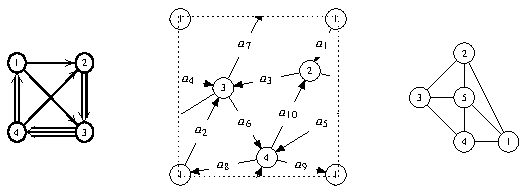
\includegraphics[width=0.86\textwidth]{figures/Fig_226_PDF329_Book317.pdf}
  \caption{Hirzebruch 曲面例中的二聚体箭图与匹配多边形（原书 p.317）}\label{fig:hirzebruch-dimer-quiver}
\end{figure}
当 $\theta=(-3,-1,2,2)$ 时，稳定完美匹配如下表所示：
\begin{center}
\begin{tabular}{c|c|c}
匹配 & 所含箭 & 格点 \\
\hline
$P_1$ & $\{9,6,4\}$ & $(1,-1)$ \\
$P_2$ & $\{7,2,10\}$ & $(0,1)$ \\
$P_3$ & $\{3,8,5\}$ & $(-1,0)$ \\
$P_4$ & $\{1,6,5\}$ & $(0,-1)$ \\
$P_5$ & $\{3,2,4\}$ & $(0,0)$
\end{tabular}
\end{center}
它们的格点在上图右侧的 Newton 多边形中以相应数字标出。奇异空间 $Y$ 是 Hirzebruch 曲面 $\Sigma_1$ 上的锥，而其消解 $Y_\theta$ 是该 Hirzebruch 曲面反典范线丛的全空间。

定理\ref{thm:ishii-ueda-toric-moduli} 还说明，环簇可分解为环面轨道之并，每个轨道参数化具有特定余支撑的表示：
\begin{itemize}
  \item 余支撑为空的表示构成稠密的三维环面轨道；
  \item 每个稳定完美匹配给出二维环面轨道，其闭包是一个环面除子；
  \item 每个稳定对给出一维环面轨道，其闭包为 $\mathbb P^1$ 或 $\mathbb A^1$；
  \item 每个稳定三元组给出一个不动点。
\end{itemize}
每个三元组 $T$ 还定义了开集 $U_T\subset Y_\theta$，它同构于 $\mathbb C^3$，并由余支撑包含于该稳定三元组的环面轨道组成。

与第\ref{subsec:one-two-three-models}节类似，$\ell$ 的零点集由除稠密轨道以外的所有轨道组成。$\ell^{-1}(0)$ 的奇点集是所有一维和零维轨道之并。我们可将奇点集
\[
  S_\theta=\operatorname{Sing}\ell^{-1}(0)
\]
视为若干 $\mathbb A^1$ 与 $\mathbb P^1$ 的并：每条内部边对应一条 $\mathbb P^1$，匹配多边形边界上的每条边对应一条 $\mathbb A^1$；对每个三角形，将其各边对应的 $\mathbb A^1$ 和 $\mathbb P^1$ 粘合于一点。每个开集 $U_T$ 上，Landau--Ginzburg 模型 $(Y_\theta,\ell)$ 限制为 $(\mathbb C^3,XYZ)$，即裤子曲面的镜像。由定理\ref{thm:tubular-graph-sheaf-functor}，$(Y_\theta,\ell)$ 的镜像可视为若干个裤子曲面的粘合；所得曲面是匹配多边形三角剖分对偶图的一个管状邻域。
\end{example}

\begin{example}[匹配多边形的分解]
继续例\ref{ex:hirzebruch-dimer-stability}。三角剖分的对偶图是一个带四条leg的四边形。奇点集 $S_\theta=\operatorname{Sing}\ell^{-1}(0)$ 由四条 $\mathbb P^1$ 和四条 $\mathbb A^1$ 组成，而镜像曲面由四枚裤子曲面粘合而成，如图\ref{fig:hirzebruch-pants-decomposition} 所示。
\begin{figure}[H]\centering
  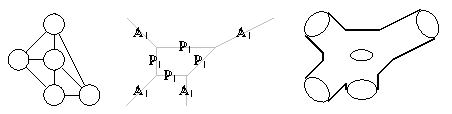
\includegraphics[width=0.52\textwidth]{figures/Fig_227_PDF331_Book319.pdf}
  \caption{Hirzebruch 例中的奇点集与裤子曲面分解（原书 p.319）}\label{fig:hirzebruch-pants-decomposition}
\end{figure}
\end{example}

另一方面，由定理\ref{thm:zigzag-consistent-dimer-mirror}，镜像也可看作对偶二聚体 $Q^\vee$ 所在的曲面，因此我们应能把该曲面切成若干裤子曲面。为此，考察对偶二聚体 $Q^\vee$ 上的完美匹配。回忆，$Q^\vee$ 是一个嵌入亏格为 $g$、有 $m$ 个标记点的曲面 $(S,M)$ 中的二聚体。亏格等于 Newton 多边形的内部格点数，标记点数等于其边界格点数。因此可将 $S\setminus M$ 识别为三角剖分对偶图 $\Gamma_\theta$ 的一个管状加厚。但如何在这一管状加厚上画出对偶二聚体的弧系？

\begin{theorem}{稳定匹配确定对偶二聚体弧系}{stable-matchings-dual-dimer-arcs}
设 $Q$ 是环面上的一致二聚体模型，$\theta$ 是通有稳定条件，$Q^\vee$ 是对偶二聚体。
\begin{enumerate}[label=(\roman*)]
  \item 对每条箭 $a$，可以在对偶图的加厚邻域上画一条分隔线，将包含 $a$ 的稳定匹配与不包含 $a$ 的稳定匹配分开。
  \item 若 $c\in Q_2$ 是一个面，则来自 $c$ 中各箭的分隔线围成一个多边形区域，该区域落在对偶图的一棵子树上。
  \item 将这些区域粘合，得到对偶图的管状邻域；这些分隔线组成的弧系表示对偶二聚体 $Q^\vee$。
\end{enumerate}
\end{theorem}
\begin{proof}[证明思路]
证明依赖二聚体的一致性，详细论证见文献\bookcite{37}。
\hfill$\square$
\end{proof}

\begin{example}[分隔线与稳定匹配]
回到 Hirzebruch 曲面的例子\ref{ex:hirzebruch-dimer-stability}。可以列出每条箭、包含它的稳定匹配及相应的分隔线；图\ref{fig:stable-matchings-separating-lines} 中标出了箭 $a_1,\ldots,a_{10}$。
\begin{figure}[H]\centering
  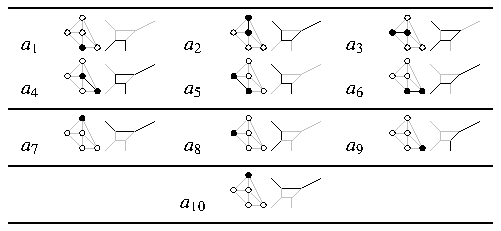
\includegraphics[width=0.7\textwidth]{figures/Fig_228_PDF332_Book320.pdf}
  \caption{稳定匹配与对偶图上的分隔线（原书 p.320）}\label{fig:stable-matchings-separating-lines}
\end{figure}

现在把 $Q^\vee$ 放到对偶图周围的管状曲面上。取稳定对 $\{P_1,P_2\}$，并取对偶图中相应边的垂直截面，得到一条简单闭曲线 $L_{P_1,P_2}$。它穿过
\[
  (P_1\cup P_2)\setminus(P_1\cap P_2)
\]
中的所有箭，并在属于 $P_1$ 的箭与属于 $P_2$ 的箭之间交替。容易在 $B$ 侧找到与这些曲线对应的对象。
\end{example}

\begin{lemma}{稳定对对应带对象}{stable-pair-band-object}
若表示 $\rho$ 的余支撑为 $P_1\cup P_2$，则在如下识别下
\[
  D_{\mathrm{Sing}}^{\pm}(\mathrm{Jac}/\langle\ell\rangle)
  \cong_\infty\mathrm{MF}^{\pm}(\mathrm{Jac},\ell)
  \cong_\infty\mathrm{topFuk}^{\pm}(S,M),
\]
$\rho$ 对应于一条底层曲线为 $L_{P_1,P_2}$ 的带对象与其平移的直和。
\end{lemma}
\begin{proof}[证明思路]
由于 $\rho$ 在 $P_1$ 上取零，矩阵分解 $M_\rho$ 可按 $2\deg_{P_1}$ 分次，因此它是弦对象与带对象的直和。它不可能含有弦对象，因为弦对象的自同态环是无限维的，而
\[
  \operatorname{Hom}^{\pm}_{\mathrm{MF}}(M_\rho,M_\rho)
  \cong\operatorname{Mat}_{2\times2}\bigl(\mathbb C[\epsilon]/(\epsilon^2)\bigr)
\]
是有限维的。这一 Hom 空间也表明，$M_\rho$ 是某条简单曲线上的带对象与其平移的直和。

此外，对箭所对应的标准矩阵分解 $M_a$ 可计算得：若 $\rho(a)=\rho(\ell a^{-1})=0$，则
\[
  \operatorname{Hom}_{\mathrm{MF}^{\pm}}(M_a,M_\rho)=\mathbb C\oplus\mathbb C;
\]
否则该 Hom 空间为零。因此，$M_\rho$ 的带对象只与那些 $P_1$ 与 $P_2$ 所取的箭不同的面中的箭相交，因为只有在这些面上，$a$ 与 $\ell a^{-1}$ 才能同时取零。由于 Hom 空间为 $\mathbb C\oplus\mathbb C$，带曲线会沿两个方向都与这些箭相交。更多细节见\bookcite{37}。
\hfill$\square$
\end{proof}

这些结果可视作某种 SYZ 纤维化：奇点集 $S_\theta$ 与曲面 $(S,M)$ 都可投影到三角剖分对偶图 $\Gamma_\theta$，如图\ref{fig:syz-over-dual-graph}。在此图中，$S_\theta$ 中的表示 $\rho$ 对应于底层曲线为
\[
  \pi_A^{-1}\bigl(\pi_B(\rho)\bigr)
\]
的带对象。图中的投影仅在同伦意义下确定，因为 $\Gamma_\theta$ 只是一个组合对象。
\begin{figure}[H]\centering
  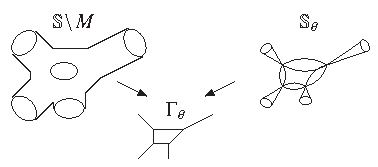
\includegraphics[width=0.66\textwidth]{figures/Fig_229_PDF333_Book321.pdf}
  \caption{奇点集与镜像曲面在对偶图上的投影（原书 p.321）}\label{fig:syz-over-dual-graph}
\end{figure}

最后，可用热带曲线将 $\Gamma_\theta$ 实现为一个实际空间。给定权函数 $w\colon Q_1\to\mathbb Z$，可定义稳定条件
\[
  \theta_w\colon Q_0\longrightarrow\mathbb Z,\qquad
  v\longmapsto\sum_{h(a)=v}w(a)-\sum_{t(a)=v}w(a).
\]
它满足 $\theta_w\cdot(1,\ldots,1)=0$；反过来，任何满足这一条件的 $\theta$ 都可由某个权函数 $w$ 实现。权函数还可定义多项式
\[
  f_{w,t}=\sum_P t^{\sum_{a\in P}w(a)}
  X^{\deg_Px}Y^{\deg_Py},
\]
其中求和遍历 $Q$ 的所有完美匹配。

\begin{theorem}{稳定匹配三角剖分的热带实现}{tropical-curve-stability-triangulation}
若 $\theta_w$ 是通有的，则其三角剖分的对偶图与 $f_{w,t}$ 的热带曲线相同。
\end{theorem}
\begin{proof}[证明思路]
热带曲线是满足下式的点 $(\xi,\eta)\in\mathbb R^2$ 的轨迹：
\[
  F^{\mathrm{trop}}(\xi,\eta)=\max_P\{L_P(\xi,\eta)\}
\]
至少由两个函数同时取到，其中
\[
  L_P(\xi,\eta)
  =(\deg_Px)\xi+(\deg_Py)\eta+\sum_{a\in P}w(a).
\]
可以证明，$P$ 为 $\theta_w$ 稳定，当且仅当存在 $(\xi,\eta)$ 使 $F^{\mathrm{trop}}(\xi,\eta)=L_P(\xi,\eta)$ 且该最大值唯一；而 $\{P_1,P_2\}$ 是稳定对，当且仅当存在 $(\xi,\eta)$ 使
\[
  F^{\mathrm{trop}}(\xi,\eta)=L_{P_1}(\xi,\eta)=L_{P_2}(\xi,\eta).
\]
因此热带曲线的边与稳定对一一对应。更多细节见\bookcite{35}。
\hfill$\square$
\end{proof}


\section{Bridgeland 稳定性}\label{sec:bridgeland-stability}

King 稳定性适用于代数的表示，但我们常常需要处理更一般的范畴或 $A_\infty$ 范畴，因此要推广稳定性的概念。为此，先用一种便于推广的方式重述 King 稳定性。
\takeaway{Bridgeland 稳定条件由中心荷 $Z\colon\Gamma\to\mathbb C$ 与切片 $\mathcal P_\phi$ 组成，五条公理保证每个对象有相位递增的半稳定锥分解；King 稳定性是 $Z(\alpha)=\theta\cdot\alpha+i\sum\alpha_v$ 的特例，稳定条件空间 $\operatorname{Stab}_\Gamma A^{\bullet}$ 是复流形，遗忘映射为局部微分同胚。}

对每个 $\theta\colon Q_0\to\mathbb Z$，可定义中心荷\index{zhongxinhe@中心荷|hyperpage}映射
\[
  Z\colon\mathbb Z^{Q_0}\longrightarrow\mathbb C,\qquad
  \alpha\longmapsto\theta\cdot\alpha+i\sum_{v\in Q_0}\alpha_v.
\]
它给每个表示 $\rho$ 赋予上半平面
\[
  \mathbb H=\{z\in\mathbb C\mid\operatorname{Im}z>0\}
\]
中的复数 $Z(\rho)$，其取值由表示的维数向量决定。表示的相位定义为
\[
  \phi(\rho)=\arg Z(\rho).
\]
按原来的定义，$\rho$ 是 $\theta$ 稳定表示，当且仅当：(i) 它的相位为 $\pi/2$；(ii) 每个真子表示的相位都小于 $\rho$ 的相位。因此，可以去掉第一个条件，得到如下定义。

\begin{definition}{表示的半稳定性}{representation-semistability}
若表示 $\rho$ 的每个真子表示的相位都小于或等于 $\phi(\rho)$，则称 $\rho$ 是相位为 $\phi(\rho)$ 的（半）稳定表示。
\end{definition}

\begin{theorem}{Harder--Narasimhan 滤过}{harder-narasimhan-filtration}
对每个表示 $\rho\colon\mathbb CQ\to\operatorname{End}(W)$，都存在滤过
\[
  0=V_0\subset V_1\subset\cdots\subset V_n=W,
\]
使每个商 $F_i=V_i/V_{i-1}$ 都是相位为 $\phi_i$ 的半稳定 $\mathbb C$-模，并且相位递减：若 $i<j$，则 $\phi_i\ge\phi_j$。这样的滤过称为 Harder--Narasimhan 滤过\index{hardernarasimhanlvguo@Harder–Narasimhan 滤过|hyperpage}。
\end{theorem}
% [Tutor Note: 定理中"半稳定 $\mathbb C$-模"应为半稳定 $\mathbb C Q$-模，即 $Q$ 的表示——原书 p.322 漏写了 $Q$，按上下文每个商 $F_i$ 都是 $\mathbb C Q$-模。]
\begin{proof}[证明思路]
对 $W$ 的总维数归纳。若维数为 $1$，则表示是简单表示，可取滤过 $0\subset W$。若 $W$ 已半稳定，也取同一滤过。

若 $W$ 不半稳定，则至少存在一个相位更大的子表示 $V_1$。取相位最大的一个，考虑 $0\subset V_1\subset W$。$V_1$ 必为半稳定，否则它包含相位更大的子表示，与 $V_1$ 的选取矛盾。同样，$W/V_1$ 不可能含有相位大于 $\phi(V_1)$ 的子表示 $V'$，否则沿自然映射 $\pi\colon W\to W/V_1$ 将 $V'$ 拉回后，其中心荷为 $Z(V_1)+Z(V')$，从而
\[
  \phi\bigl(\pi^{-1}(V')\bigr)>\phi(V_1),
\]
仍与 $V_1$ 的最大性矛盾。由归纳假设，$W/V_1$ 有相位递减的滤过
\[
  0\subset V'_2\subset\cdots\subset V'_k=W/V_1.
\]
这些表示的拉回 $V_i=\pi^{-1}(V'_i)$ 仍按相位递减，故
\[
  0\subset V_1\subset V_2\subset\cdots\subset V_k
  =\pi^{-1}(V'_k)=W
\]
即为所求滤过。
\hfill$\square$
\end{proof}

\begin{figure}[H]\centering
  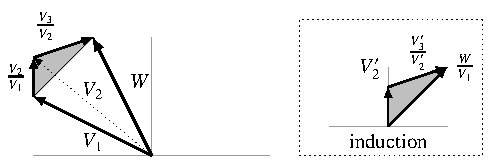
\includegraphics[width=0.88\textwidth]{figures/Fig_230_PDF335_Book323.pdf}
  \caption{Harder--Narasimhan 滤过的中心荷分解与归纳步骤（原书 p.323）}\label{fig:harder-narasimhan-central-charge}
\end{figure}

\begin{note}[Harder--Narasimhan 滤过的适用范围]
Harder--Narasimhan 滤过的存在并不限于箭图表示；它对向量丛分类也很重要（该术语最初即源于向量丛理论\bookcite{193,117}）。若 $E$ 是一条曲线、$V$ 是其上的向量丛，可定义中心荷
\[
  Z(V)=-\deg V+i\,\operatorname{rk}V,
\]
并将相位取为 $\arg Z(V)\in(0,\pi]$。
\end{note}

\begin{note}[相位与斜率]
文献中通常使用斜率而非相位。斜率是
\[
  \mu=\frac{\deg V}{\operatorname{rk}V}
\]
（对箭图表示则为 $\mu=-\theta\cdot\alpha/\sum_v\alpha_v$，见\bookcite{112,207}）。二者等价，因为有单调关系
\[
  \phi=\arctan(\mu)+\frac{\pi}{2}.
\]
与斜率相比，相位的优点在于可以推广到表示的整个导出范畴 $D\mathrm{mod}^{\bullet}Q$。我们把 $Z$ 视为从（数值）格罗滕迪克群到 $\mathbb C$ 的映射。若 $\rho$ 是相位为 $\phi(\rho)$ 的半稳定表示，则称 $\rho[k]$ 是相位为 $\phi(\rho)+k\pi$ 的半稳定对象。按此约定，$D\mathrm{mod}^{\bullet}Q$ 中所有对象都可表示为相位递增的半稳定对象的锥。
\end{note}

要把这些想法推广到 $A_\infty$ 范畴，需要将 Bridgeland\bookcite{39}为三角范畴发展的稳定条件重述到扭曲完备的 $A_\infty$ 范畴中。关键在于把滤过改写为扭曲复形。若
\[
  V_0\subset\cdots\subset V_k
\]
是滤过，则 $V_k$ 是一系列扩张锥，可写成扭曲复形
\[
  V_k=\left(\bigoplus_{i=1}^k V_i/V_{i-1},
  \alpha_k+\alpha_{k-1}+\cdots+\alpha_1\right),
\]
其中 $\alpha_i$ 是相应短正合列
\[
  0\longrightarrow V_{i-1}/V_{i-2}
  \longrightarrow V_i/V_{i-2}
  \longrightarrow V_i/V_{i-1}\longrightarrow0
\]
所对应的扩张态射。因此，滤过的因子相位递减，对应于直和项相位递增的扭曲复形。

\begin{definition}{Bridgeland 稳定条件}{bridgeland-stability-condition}
设 $A^{\bullet}$ 是扭曲完备的极小 $A_\infty$ 范畴，并固定群同态
\[
  v\colon K_0A^{\bullet}\longrightarrow\Gamma,
\]
其中 $\Gamma\cong\mathbb Z^N$ 是有限生成自由阿贝尔群。一个 Bridgeland 稳定条件\index{bridgelandwendingtiaojian@Bridgeland 稳定条件|hyperpage}由二元组 $(Z,\mathcal P)$ 组成：$Z\colon\Gamma\to\mathbb C$ 是称为中心荷的群同态；对每个 $\phi\in\mathbb R$，$\mathcal P_\phi$ 是 $A^{\bullet}$ 的满加法子范畴，其对象称为相位 $\phi$ 的半稳定对象。该二元组需满足以下公理。
\begin{enumerate}[label=(SC\arabic*)]
  \item \textbf{中心荷与相位。}对任意 $X\in\mathcal P_\phi$，若 $X\ne0$，则
  \[
    Z(X)\in\mathbb R_{>0}e^{i\phi}.
  \]
  这里以 $Z(X)$ 简记 $Z(v[X])$。
  \item \textbf{平移。}平移使相位增加 $\pi$：
  \[
    \mathcal P_{\phi+\pi}=\mathcal P_\phi[1].
  \]
  \item \textbf{态射与相位。}若 $X_1\in\mathcal P_{\phi_1}$、$X_2\in\mathcal P_{\phi_2}$ 且 $\phi_1>\phi_2$，则
  \[
    A^0(X_1,X_2)=0.
  \]
  \item \textbf{锥分解。}每个对象都是相位递增的半稳定对象的迭代锥：对每个 $X\in A^{\bullet}$，存在 $\phi_1<\cdots<\phi_k$ 及 $X_i\in\mathcal P_{\phi_i}$，使得
  \[
    X\cong(X_1\oplus\cdots\oplus X_k,\delta).
  \]
  可以证明，对给定的 $X$，这些 $X_i$ 在拟同构意义下唯一确定。记
  \[
    \phi^-(X)=\phi_1,\qquad\phi^+(X)=\phi_k.
  \]
  \item \textbf{支撑性质\index{zhichengxingzhi@支撑性质|hyperpage}。}中心荷不能在半稳定对象上任意趋近于零：存在常数 $C>0$，使对所有非零半稳定对象 $X$，都有
  \[
    \|v([X])\|\le C|Z(X)|,
  \]
  其中 $\|\cdot\|$ 是 $\mathbb Z^N$ 上的标准范数。
\end{enumerate}
\end{definition}
% [Tutor Note: (SC4) 中的 $X_i$ 在拟同构意义下唯一，这保证 $\phi^{\pm}(X)$ 与心 $\heartsuit_\sigma$ 良定义；切片按 $\pi$ 周期（见 (SC2)），故 (SC4) 里的相位可以整体平移 $\pi$ 的整数倍，实际只用到 $(0,\pi]$ 这一段，心也正是为此取成半开区间。]

\begin{note}[支撑性质]
Bridgeland 原始定义中没有群 $\Gamma$，而是直接使用整个格罗滕迪克群；证明其主要结果定理\ref{thm:bridgeland-manifold} 时使用的是另一条性质——局部有限性，而非公理 (SC5)。然而，格罗滕迪克群不一定有限生成，这会导致稳定条件空间无穷维。为控制格罗滕迪克群的规模，可引入同态 $v$；文献\bookcite{149}将公理 (SC5) 作为支撑性质提出。关于该性质及其意义的进一步讨论，见\bookcite{30}。
\end{note}

\begin{note}[心与子对象]
注意，在模范畴 $\mathrm{Mod}^{\bullet}R$ 中，映射 $f$ 是单射，当且仅当锥
\[
  \operatorname{Cone}(f\colon X[-1]\to Y)\in D\mathrm{Mod}^{\bullet}R
\]
同构于一个模（等价地，其上同调集中在次数 $0$）。此时 $f$ 将 $X$ 嵌入 $Y$，而该锥是 $f$ 的余核。

一般的 $A_\infty$ 范畴没有子对象或商对象的概念，可借助切片来处理。给定稳定条件 $\sigma=(Z,\mathcal P)$，定义其心\index{wendingtiaojiandexin@稳定条件的心|hyperpage} $\heartsuit_\sigma$ 为所有满足
\[
  \phi^+(X),\phi^-(X)\in(0,\pi]
\]
的对象所成的子范畴。若 $X,Y\in\heartsuit_\sigma$，且 $f\colon X\to Y$ 是次数为 $0$ 的映射，并且
\[
  \operatorname{Cone}(f\colon X[-1]\to Y)\in\heartsuit_\sigma,
\]
则称 $f$ 是嵌入，并称 $X$ 是 $Y$ 的子对象。

心和中心荷足以重建所有切片。对 $\phi\in(0,\pi]$，切片 $\mathcal P_\phi$ 由心中的对象 $Y$ 构成，这些对象满足 $Z(Y)\in\mathbb R_{>0}e^{i\phi}$，且不存在一个子对象 $X$ 使 $Z(X)\in\mathbb R_{>0}e^{i\phi'}$ 且 $\phi'>\phi$。由此得到把稳定条件公理化为一对 $(Z,\heartsuit)$ 的另一种方式。更多细节见\bookcite{40}。
\end{note}

\begin{example}[线性箭图上的稳定条件]
设 $Q$ 是线性箭图，考虑 $D\mathrm{mod}^{\bullet}Q$。第四章中，我们把它解释为一个 $(n+1)$ 边形的边与对角线所成的范畴。将此多边形嵌入 $\mathbb C$ 为一个凸 $(n+1)$ 边形，并在 $\mathbb C$ 上取水平线场，则每个不可分解对象都可视为一个带相位角的复向量。将每条线段映到其向量即可定义中心荷；令 $\mathcal P_\phi$ 为由相位为 $\phi$ 的不可分解对象的所有直和组成的范畴。其构造见图\ref{fig:linear-quiver-stability}。
\begin{figure}[H]\centering
  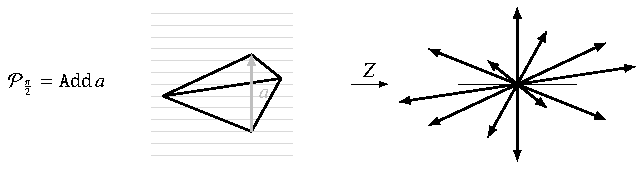
\includegraphics[width=0.75\textwidth]{figures/Fig_231_PDF337_Book325.pdf}
  \caption{凸多边形给出的线性箭图稳定条件（原书 p.325）}\label{fig:linear-quiver-stability}
\end{figure}
容易验证，这五条稳定性公理均成立：(SC1)、(SC2) 来自分次的定义；(SC3) 成立，因为所有态射都可看成相位在 $(0,\pi)$ 内的正角；(SC4) 成立，因为可按相位排列不可分解直和项并取平凡的 $\delta$；最后，因不可分解对象只有有限多个，(SC5) 也成立。

现在将凸多边形的一个顶点向内移动，直至多边形变成凹多边形。此时稳定条件会怎样变化？与该点相邻的两条边的相位逐渐趋同，随后交换次序。发生交换时，伸到多边形之外的对角线相位小于第一条边，因此它们之间的态射从高相位对象指向低相位对象。可将该对角线声明为不稳定对象，从而解决这个问题，见图\ref{fig:concave-quiver-stability}。
\begin{figure}[H]\centering
  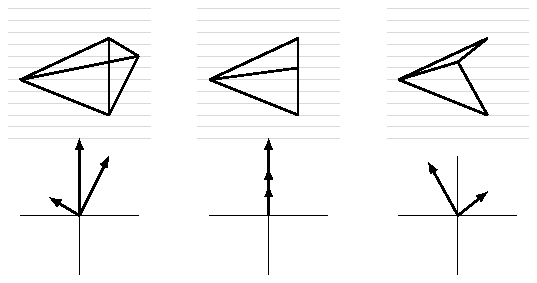
\includegraphics[width=0.81\textwidth]{figures/Fig_232_PDF338_Book326.pdf}
  \caption{顶点移动后不稳定的对角线（原书 p.326）}\label{fig:concave-quiver-stability}
\end{figure}
这样处理后，Harder--Narasimhan 性质仍成立：不稳定对角线是两条边的锥；由于两条边的相位顺序已交换，它确实是相位递增对象之间的锥。

这个例子表明，给定稳定条件 $(Z,\mathcal P)$，可以连续地向各个方向改变中心荷，并在过程中相应改变切片 $\mathcal P_\phi$。下面的定理准确表达这一点。
\end{example}

\begin{theorem}{Bridgeland 稳定条件空间定理}{bridgeland-manifold}
\textnormal{（Bridgeland）}给定 $A_\infty$ 范畴 $A^{\bullet}$ 及映射 $v\colon K_0A^{\bullet}\to\Gamma$，稳定条件集合 $\operatorname{Stab}_\Gamma A^{\bullet}$ 可赋予复流形结构，使遗忘映射
\[
  \operatorname{Stab}_\Gamma A^{\bullet}
  \longrightarrow\operatorname{Grp}(\Gamma,\mathbb C),
  \qquad (Z,\mathcal P)\longmapsto Z
\]
成为局部微分同胚。
\end{theorem}
\begin{proof}[证明思路]
Bridgeland 对三角范畴给出的原始定理（未引入额外映射 $v$，并使用局部有限稳定条件）的证明见\bookcite{39}。支撑性质的相关讨论见\bookcite{30}附录 A。其核心是：当 $Z$ 发生微小变化时，要控制稳定对象的相位。若 $K_0A^{\bullet}$ 有限生成，可取 $\Gamma=K_0A^{\bullet}$，并省去下标。
\hfill$\square$
\end{proof}

\begin{note}[稳定流形的连通分支]\label{note:stability-manifold-components}
一般而言，描述一个范畴的整个稳定流形并不容易；但给定一个稳定条件，有时可以描述它所在的连通分支。在少数情况下，还能证明稳定流形是连通的，从而得到完整描述。
\end{note}

\begin{note}[自等价群对稳定流形的作用]\label{note:stability-manifold-autoequivalences}
若 $\mathcal F\colon A^{\bullet}\to A^{\bullet}$ 是范畴的自等价，它会在稳定流形上诱导一个同胚。因此，稳定流形带有范畴自同构群的作用，也可以考察商空间 $\operatorname{Stab}(A^{\bullet})/\operatorname{Aut}A^{\bullet}$。稳定条件空间本身往往是可缩的，但这个商空间可能具有丰富的拓扑结构。
\end{note}


\section{稳定条件与二次微分}\label{sec:stability-quadratic-differentials}

上一节线性箭图的例子说明：可以把多边形与复平面的一部分等同，从而构造稳定条件。本节把这一想法推广到带一形式或二次微分的曲面。Bridgeland--Smith\bookcite{44} 和 Sutherland\bookcite{233} 最先用二次微分构造稳定条件：前者处理曲面，后者处理三维 Calabi--Yau（CY3）代数；Haiden、Katzarkov 和 Kontsevich\bookcite{115} 处理了曲面 Fukaya 范畴的情形。本节展示其中若干例子，下一节讨论其主要结果。
\takeaway{把多边形嵌入复平面、或沿曲面积分一形式 $\omega$（二次微分则取 $\sqrt{\varphi}$ 提升到双覆盖上），可定义中心荷；特殊曲线是平直度量下相位恒定的直线，射线叶把曲面切成有限与无限条带，由此构造稳定条件并把 Harder--Narasimhan 分解解释为曲线的拉直过程。}

先看略简单的一形式情形。设 $(\vec S,M)$ 是没有边界、分次来自一形式 $\omega$ 的分次曲面，且 $\omega$ 的零点与极点都位于 $M$。对 $\mathrm{topFuk}^{\bullet}(\vec S,M)$ 中的每个对象 $L$，沿其底层曲线积分可赋予一个复数：
\[
  Z(L)=\int_0^1\omega(\dot{\vec L}(t))\,dt,
\]
其中 $\vec L(t)$ 是对象所代表曲线的一种参数化。该数只依赖 $\vec L$ 的同调类，故 $Z(L)$ 定义良好，但可能为无穷大；当弦的起点或终点是 $\omega$ 的极点时就会发生这种情况。令 $\Gamma\subset H_1(\vec S,M)$ 为由避开这些极点的弦与带的同调类生成的子群，则 $Z$ 可看成中心荷 $Z\colon\Gamma\to\mathbb C$。再令
\[
  {}^{\mathrm{fin}}\mathrm{Fuk}^{\bullet}(\vec S,M)
  \subset\mathrm{topFuk}^{\bullet}(\vec S,M)
\]
为由避开这些极点的弦对象和带对象生成的子范畴，则有自然映射
\[
  v\colon{}^{\mathrm{fin}}\mathrm{Fuk}^{\bullet}(\vec S,M)\longrightarrow\Gamma,
\]
将弦或带对象映到其同调类。

要选出半稳定对象，先定义曲线长度
\[
  \ell(\vec L):=\int_0^1|\omega(\dot{\vec L}(t))|\,dt.
\]
由三角不等式，$|Z(L)|\le\ell(\vec L)$；若取等号，则称 $\vec L$ 为特殊曲线。该长度给 $S\setminus M$ 赋予平直度量，因为每个点 $p\in S\setminus M$ 附近都可取局部复坐标 $z$，使得 $\omega=dz$。写 $z=x+iy$ 后，长度公式正是欧氏长度。

因此可把特殊曲线看作直线。分次拉格朗日曲线的相位函数为常数，并且模 $\pi$ 后等于 $\arg Z(L)$。这是具体曲线的性质，而非其同伦类的性质：一个同伦类中可能有特殊曲线，也可能没有。若对象 $L$ 可由特殊曲线 $\vec L$ 表示，则称其为相位 $\phi=\theta$ 的半稳定对象。由此得到切片 $\mathcal P_\phi$。
% [Tutor Note: 特殊曲线的相位就是它在平直度量下的方向角：$\int\omega$ 给出的复向量方向恒定，而 $|Z(L)|\le\ell(\vec L)$ 取等号当且仅当曲线处处沿该方向前进。所以这里判断稳定性是纯几何的：把曲线在同伦类中拉直到最短，得到的折线段就给出 Harder--Narasimhan 分解。]

对任意曲线 $\vec L$，可以通过改变曲线使长度尽可能短。曲线通常会逐渐变直，但有时会被标记点挡住；此时极限会成为若干折线段，并且弦或带对象可看作这些折线段的锥。角态射的次数为 $1$，但转过的角度大于 $\pi$，所以锥中的直和项相位递增，正对应于 Harder--Narasimhan 滤过。
\begin{figure}[H]\centering
  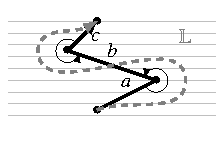
\includegraphics[width=0.32\textwidth]{figures/Fig_233_PDF340_Book328.pdf}
  \caption{曲线缩短过程中的折线分解（原书 p.328）}\label{fig:broken-line-hn}
\end{figure}
支撑性质的验证见\bookcite{115}第 5.4 节。

\begin{example}[对数一形式给出的稳定对象]
取标记点为 $\{0,1,2,\infty\}$ 的 Riemann 球面，并令
\[
  \omega=\frac{dz}{z}=d\ln z.
\]
相应线场的叶是径向直线。若弧起点或终点为 $0$ 或 $\infty$，其长度为无穷大。从 $1$ 出发、终止于 $2$ 并在环带 $1<|z|<2$ 中绕一圈的弧，其中心荷为
\[
  \int_{\vec L}d\ln z=\ln 2+2\pi i=:u.
\]
它可由特殊拉格朗日曲线 $\gamma(t)=e^{ut}$ 表示，相位为 $\theta=\arctan(2\pi/\ln 2)$，因此是稳定对象，见图\ref{fig:logarithmic-form-stable-arc}。
\begin{figure}[H]\centering
  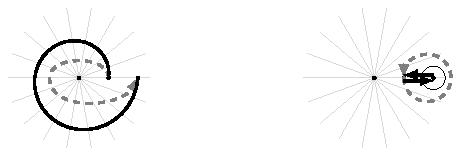
\includegraphics[width=0.74\textwidth]{figures/Fig_234_PDF341_Book329.pdf}
  \caption{对数一形式下的稳定弧与不稳定弧（原书 p.329）}\label{fig:logarithmic-form-stable-arc}
\end{figure}

从 $1$ 出发又回到 $1$、绕过 $2$ 但不绕环带的弧，其中心荷为 $0$，因此不可能稳定。它分解为
\[
  (a\oplus a[1],\alpha),
\]
其中 $a$ 是从 $1$ 到 $2$ 的简单直弧，$\alpha$ 是绕 $2$ 的整周角。
\end{example}

若使用二次微分 $\varphi$ 代替一形式，也可以作同样构造，只需对 $\varphi$ 取平方根。由于我们在复数域上工作，平方根一般不是 $S$ 上的一形式，而是双覆盖 $\widetilde S$ 上的一形式。每条曲线 $L$ 都提升为 $\widetilde L$，并可在覆盖空间上积分。

\begin{example}[二次微分的双覆盖]
取 Riemann 球面 $S=\widehat{\mathbb C}$、标记点 $\{-1,1,\infty\}$ 及二次微分
\[
  \varphi=\frac{dz^2}{1-z^2}.
\]
水平线场由连接 $-1$ 与 $1$ 的直线及其周围的椭圆组成（见例\ref{ex:sphere-arc-grading}）。沿映射
\[
  z=\frac12(u+u^{-1})
\]
拉回 $\varphi$ 后得到 $-u^{-2}du^2$，因此可取平方根 $\sqrt{\varphi}=iu^{-1}du$。该映射是一个双覆盖，在 $z=\pm1$ 处分支而在 $z=\infty$ 处不分支；所得覆盖曲面是带四个标记点的球面，可识别为带一形式 $i\,du/u$ 的 $(\mathbb P^1,\{0,1,-1,\infty\})$，如图\ref{fig:quadratic-differential-double-cover}。
\begin{figure}[H]\centering
  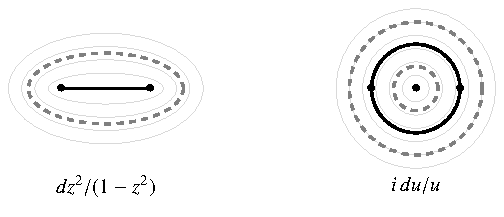
\includegraphics[width=0.75\textwidth]{figures/Fig_235_PDF341_Book329.pdf}
  \caption{二次微分及其双覆盖上的一形式（原书 p.329）}\label{fig:quadratic-differential-double-cover}
\end{figure}

连接 $-1$ 和 $1$ 的直线提升为单位圆上连接 $1$ 与 $-1$ 的两段半圆弧，提升后的总中心荷为 $2\pi$。每条椭圆提升为两个圆，一个在单位圆内，一个在单位圆外，总中心荷为 $4\pi$。相应的弦对象与带对象的相位均为 $0$（因为中心荷为实数）。利用双覆盖上的中心荷与相位，即可为 ${}^{\mathrm{fin}}\mathrm{Fuk}^{\bullet}(\vec S,M)$ 构造稳定条件。
\end{example}
% [Tutor Note: 平方根 $\sqrt{\varphi}$ 只有在双覆盖 $\widetilde S$ 上才是整体一形式，双覆盖在 $\varphi$ 的零点与极点处分枝；因此中心荷要在覆盖上积分后再取，长度也相应翻倍——例中直线提升后的总中心荷为 $2\pi$、椭圆为 $4\pi$，正是这个原因。]

每个定义在 $(S,M)$ 上的二次微分 $\varphi$ 都确定两种结构：水平叶状结构和度量。该叶状结构的叶是此度量下相位恒为 $0$ 的测地线。根据端点类型，叶可分为：
\begin{itemize}
  \item \textbf{闭叶：}没有端点；
  \item \textbf{有限叶：}连接两个形如 $z^kdz^2$、$k\ge-1$ 的标记点（即其绕数为正）的叶，长度有限；
  \item \textbf{射线叶：}从一个满足 $k\ge-1$ 的标记点出发，终止于一个满足 $k<-1$ 的标记点；它在一端长度有限，在另一端长度无穷；
  \item \textbf{无限叶：}连接两个形如 $z^kdz^2$、$k<-1$ 的标记点，长度无穷。
\end{itemize}
如例\ref{ex:quadratic-differential-line-fields} 所示，每个满足 $z^kdz^2$、$k\ge-1$ 的标记点都有 $k+2$ 个有限叶端点抵达，其切向方向为
\[
  e^{2\pi ir/(k+2)}.
\]
因此，射线叶和有限叶的数量有上界。

有限叶的出现是特殊现象，因为它要求两个有限端点恰好相遇。可以证明，若至少有一个标记点的绕数为正，则稍微旋转二次微分为 $e^{i\epsilon}\varphi$ 后，可以消除所有闭叶和有限叶。此时沿射线叶切开曲面。相邻射线叶之间的角度为 $\pi$，因此相邻射线共同组成一条直线。所得各部分与下列条带同胚：
\[
  S_r=\left(\{x+iy\in\mathbb C\mid0<y<r\},(dz)^2\right),
  \qquad r\in(0,+\infty].
\]
若 $r<\infty$，称为有限条带，其两侧边界由两条射线组成，分别在标记点 $m_1=x_1$、$m_2=x_2+ri$ 相遇；若 $r=\infty$，称为无限条带，其下边界由两条射线组成。

\begin{example}[有限叶分裂为射线]
回到上一例。二次微分 $\varphi=dz^2/(1-z^2)$ 有一条有限叶；若将它微调为 $e^{i\epsilon}dz^2/(1-z^2)$，该有限叶便分裂为两条通向无穷远的射线。沿射线切开后得到一条有限条带，其每一侧都由同一条射线的两份边界围成，如图\ref{fig:finite-leaf-strip}。
\begin{figure}[H]\centering
  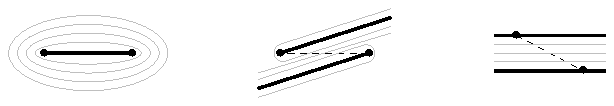
\includegraphics[width=0.93\textwidth]{figures/Fig_236_PDF342_Book330.pdf}
  \caption{有限叶旋转后分裂为射线（原书 p.330）}\label{fig:finite-leaf-strip}
\end{figure}
\end{example}

\begin{example}[含有限条带与无限条带的分解]
考虑带标记点 $\{0,\infty\}$ 的 Riemann 球面 $\widehat{\mathbb C}$，并取二次微分 $\varphi=z(dz)^2$。从 $0$ 出发有三条射线叶通向 $\infty$，切开曲面后得到三条无限条带。再在 $1\in\widehat{\mathbb C}$ 添加一个标记点，则实方向上的叶在该点处分成两段，形成一条有限叶。稍微旋转 $\varphi$ 后，这条有限叶避开 $1$ 并成为射线。包含 $1$ 的楔形区域分成两块：一块是有限条带，其另一端由经过 $1$ 的叶（现在分成两条射线）围成；另一块是无限条带，见图\ref{fig:finite-infinite-strips}。
\begin{figure}[H]\centering
  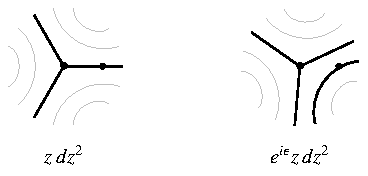
\includegraphics[width=0.58\textwidth]{figures/Fig_237_PDF343_Book331.pdf}
  \caption{添加标记点前后的条带分解（原书 p.331）}\label{fig:finite-infinite-strips}
\end{figure}
\end{example}

上述例子说明，如何为有内部标记点且没有边界分支的分次曲面构造稳定条件。若要包含边界分支，则需考察带有指数奇点的二次微分。

\begin{example}[指数二次微分]
考虑 $\mathbb C$ 上的二次微分
\[
  \varphi=e^{f(z)}dz^2,
\]
其中 $f(z)$ 是 $n$ 次多项式。先取 $f(z)=z$。水平线场由高度为 $2k\pi$ 的水平直线与夹在它们之间的弯曲线组成；每条弯曲线从 $+\infty+2k\pi i$ 出发，转弯后回到 $+\infty+2(k+1)\pi i$。

若将 $\mathbb C$ 径向压缩到单位圆盘内，每条水平直线变成连接 $-1$ 与 $1$ 的曲线；夹在其中的弯曲线变成从 $1$ 出发又回到 $1$ 的叶瓣，其长度为无穷大。另一方面，圆盘内任意以 $-1$ 为起点或终点的曲线长度都有限。图\ref{fig:exponential-quadratic-differentials} 展示了 $e^z dz^2$ 与更高次数情形。
\begin{figure}[H]\centering
  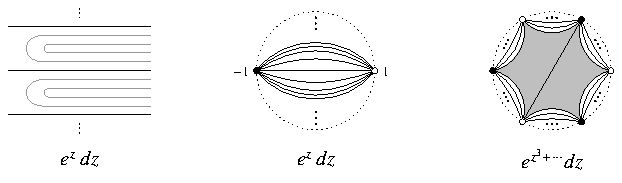
\includegraphics[width=0.98\textwidth]{figures/Fig_238_PDF343_Book331.pdf}
  \caption{指数二次微分在圆盘中的叶状结构（原书 p.331）}\label{fig:exponential-quadratic-differentials}
\end{figure}

若 $f(z)=z^n+\cdots$，则在 $|z|\gg0$ 时，该图景展开 $n$ 次。一般位置下，水平射线从 $-1$ 的 $n$ 次方根出发，终止于 $1$ 的 $n$ 次方根；$f$ 的低次项决定它们分别终止于哪些根（在非一般情形下，也可能出现连接两个 $-1$ 的根的射线）。任何从 $-1$ 的某个根出发、又终止于另一个 $-1$ 的根的曲线都具有有限长度。因此，可用该二次微分计算圆盘上带 $n$ 个标记点（即 $-1$ 的 $n$ 次方根）的分次线段的中心荷。

此外，长度等于中心荷范数的曲线称为稳定曲线。由此可在带 $n$ 个标记点的圆盘 Fukaya 范畴上得到稳定条件。与闭曲面上的二次微分一样，可以将圆盘内部连同标记点作条带分解。射线叶是从 $-1$ 的根出发的直线；这类射线有无穷多条，因而条带也有无穷多条。只有有限多个条带是有限条带（图中灰色部分）；其余都是无限条带，可以忽略，因为标记点之间的任意曲线都有代表元落在这些条带之外（也就是灰色区域内）。
\end{example}

\begin{note}[多边形的核心]
由指数二次微分得到的稳定条件与将多边形嵌入欧氏平面所得的基本稳定条件有何关系？后者是前者的特例。先过多边形每个顶点画水平直线，再在每个顶点外侧接上两列无限条带，组成鞍形楔形花束。所得对象可解释为一个带指数二次微分的曲面。将其投影到圆盘后，水平射线会变成直线：它们从一个 $-1$ 的根出发，终止于射线所交多边形边两端的 $-1$ 的根之间的那个根。
\begin{figure}[H]\centering
  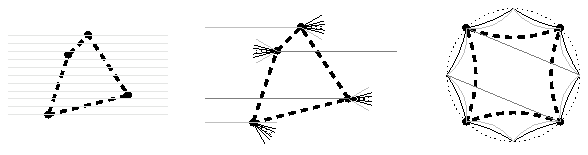
\includegraphics[width=0.90\textwidth]{figures/Fig_239_PDF344_Book332.pdf}
  \caption{由指数二次微分恢复多边形核心（原书 p.332）}\label{fig:polygon-core-from-differential}
\end{figure}

由二次微分重建多边形时，取标记点的凸包，即包含这些点且对取直线段运算封闭的最小子集（直线按二次微分的度量定义）。该集合也称为二次微分的核心\index{erciweifendehexin@二次微分的核心|hyperpage}。有些二次微分的核心是凸多边形，但并非总是如此。图\ref{fig:polygon-core-from-differential} 示意了此构造。
\end{note}

\begin{note}[平移对稳定条件的影响]
设 $\gamma$ 是 $\mathbb C$ 中的一条曲线，其在圆盘中的像连接圆周上的两个标记点。将该曲线平移常数 $c$，不会改变它的中心荷或稳定性。因此，二次微分
\[
  \varphi=e^{f(z)}dz^2,\qquad \varphi=e^{f(z-c)}dz^2
\]
定义相同的稳定条件。
\end{note}


\section{稳定流形}\label{sec:stability-manifolds}

我们已经看到，二次微分可用于为分次曲面的 Fukaya 范畴构造稳定条件。在大多数情形下，这个方法足以描述整个稳定流形。
\takeaway{二次微分给出的稳定条件由平直结构空间 $\mathrm{Flat}(S^{\flat})$ 参数化，$\iota$ 是开闭嵌入，故它恰为一个连通分支；线性箭图、射影直线与四标记球面的例子分别算出 $\mathbb C^n$、$\mathbb C^2$、$\mathbb C\times\mathbb H^+$ 型分支，Takeda 定理给出 $\mathrm{Flat}=\operatorname{Stab}$ 的充分条件。}

设 $(S,M)$ 是没有边界的紧致带标记曲面。给 $S$ 一个复结构 $J\colon TS\to TS$，并取二次微分
\[
  \varphi\in(T^*_{\mathbb C}S)^{\otimes2},
\]
要求它在 $S\setminus M$ 上处处有定义且非零。还假设每个标记点至多是指数奇点：对每个 $m\in M$，存在以 $m$ 为原点的局部复坐标 $z$，使得
\[
  \varphi=e^{z^{-n}}z^kf(z)\,dz^2,
\]
其中 $n\in\mathbb Z_{\ge0}$、$k\in\mathbb Z$，且 $f(z)$ 是满足 $f(0)\ne0$ 的全纯函数。
\begin{itemize}
  \item 若 $n>0$，称该点为 $(n,k)$ 型指数极点\index{zhishujidian@指数极点|hyperpage}。其邻域内有 $n$ 条特殊水平叶从使 $z^n$ 为负实数的方向趋近该点；这些叶在该点附近长度有限。
  \item 若 $n=0$ 且 $k<-1$，称该点为高阶极点\index{gaojiejidian@高阶极点|hyperpage}。所有水平叶在这些点附近的长度都无穷大。
\end{itemize}
数据 $S^{\flat}=(S,M,J,\varphi)$ 有时称为带锥形奇点的平\index{daizhuixingqidiandepingtanqumian@带锥形奇点的平坦曲面|hyperpage}直曲面。对每个 $(n,k)$ 型指数标记点，切去一个小圆盘，并在特殊水平叶与圆周的交点处添上 $n$ 个新标记点。所得新带标记曲面记为 $(\vec S^{\circ},M^{\circ})$；可将二次微分诱导的线场限制到其上，从而为其赋予分次。记其相对同调群为
\[
  \Gamma=H_1(\vec S^{\circ},M^{\circ}).
\]

\begin{definition}{平直曲面的 Fukaya 范畴与稳定条件空间}{flat-surface-fukaya-stability}
$\mathrm{Fuk}^{\bullet}(S^{\flat})$ 是 $\mathrm{topFuk}^{\bullet}(\vec S^{\circ},M^{\circ})$ 的子范畴，由带对象及端点不在高阶极点上的弦对象生成。存在自然映射
\[
  v\colon K_0\mathrm{Fuk}^{\bullet}(S^{\flat})\longrightarrow\Gamma.
\]
记这一映射对应的稳定条件空间为
\[
  \operatorname{Stab}(S^{\flat})
  :=\operatorname{Stab}_{\Gamma}\mathrm{Fuk}^{\bullet}(S^{\flat}).
\]
\end{definition}

显然，$(J,\varphi)$ 本身确定了 $\operatorname{Stab}(S^{\flat})$ 中的一个稳定条件 $\sigma$。其中心荷由积分 $\sqrt\varphi$ 得到，并令围绕指数极点的小圆周半径趋于零。切片 $\mathcal P_\phi$ 由那些可由相位恒为 $\phi$ 的分次曲线表示的对象生成。

设有一族平直曲面
\[
  S_t^{\flat}=(S,M,J_t,\varphi_t)_{t\in[0,1]},
\]
且 $S_0^{\flat}=S^{\flat}$，并保持 $M$ 中零点和极点的类型不变。也保持指数极点处的有限个入射方向，从而保持小圆上的标记点不变。于是 $(S^{\circ},M^{\circ})$ 不变，分次线场彼此同位；曲线的分次也可沿这族曲面传递，从而得到等价
\[
  I\colon\mathrm{Fuk}^{\bullet}(S_0^{\flat})
  \longrightarrow\mathrm{Fuk}^{\bullet}(S_1^{\flat}).
\]
例如，对曲面族 $(S,M,J,e^{2\pi it}\varphi)_{t\in[0,1]}$，该等价对应于 $\mathrm{Fuk}^{\bullet}(S^{\flat})$ 上的平移函子。

函子 $I$ 可将 $\mathrm{Fuk}^{\bullet}(S_1^{\flat})$ 上的标准稳定条件拉回为 $\mathrm{Fuk}^{\bullet}(S^{\flat})$ 上的稳定条件，得到
\[
  I^*\sigma_{S_1^{\flat}}\in\operatorname{Stab}(S^{\flat}),
\]
它只依赖于曲面族的同伦类。此外，若 $\tau_t\colon S\to S$ 是一族固定标记点的微分同胚，且 $\tau_0=1_S$，则曲面族 $\tau_t^*S_t^{\flat}$ 与 $S_t^{\flat}$ 给出相同的稳定条件。

因此，要描述由此得到的全部稳定条件，可考察 $(S,M)$ 上平直结构模空间（按微分同胚取商）的万有覆盖。记包含 $S^{\flat}$ 的连通分支为 $\mathrm{Flat}(S^{\flat})$。该空间每个点对应于一个始于 $S^{\flat}$ 的平直结构族，因而得到映射
\[
  \iota\colon\mathrm{Flat}(S^{\flat})\longrightarrow\operatorname{Stab}(S^{\flat}),
  \qquad [S_t^{\flat}]\longmapsto I^*\sigma_{S_1^{\flat}}.
\]

\begin{theorem}{平直结构与稳定条件}{flat-structures-stability-component}
\textnormal{（Haiden--Katzarkov--Kontsevich）}映射 $\iota$ 是开闭嵌入。换言之，$\mathrm{Flat}(S^{\flat})$ 是 $\operatorname{Stab}(S^{\flat})$ 的一个连通分支。
\end{theorem}
\begin{proof}[证明思路]
对任一平直曲面 $S_0^{\flat}=(S,M,J,\varphi)$，可找到 $e^{i\epsilon}\in\mathbb C^*$，使 $(S,M,J,e^{i\epsilon}\varphi)$ 可由有限和无限水平条带粘合而成，并且每条边界上恰有一个标记点。每条条带两侧标记点之间的复向量
\[
  a_j=h_j+iw_j
\]
确定该平直曲面。因此，在 $S_0^{\flat}$ 附近，平直结构空间由向量 $e^{-i\epsilon}(h_j+iw_j)$ 局部描述，见图\ref{fig:strip-flat-structure-coordinates}。
\begin{figure}[H]\centering
  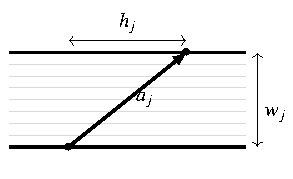
\includegraphics[width=0.42\textwidth]{figures/Fig_240_PDF346_Book334.pdf}
  \caption{条带的复坐标与平直结构局部参数（原书 p.334）}\label{fig:strip-flat-structure-coordinates}
\end{figure}

每条有限条带都包含一条连接其两侧标记点的稳定弧，其中心荷是两个复点之差。由于这些弧生成 $\Gamma$，复数 $e^{-i\epsilon}(h_j+iw_j)$ 确定 $S_0^{\flat}$ 附近稳定条件的中心荷。因此 $\iota$ 是局部同胚。关于其像开闭且映射单射的证明，参见\bookcite{115}。
\hfill$\square$
\end{proof}
% [Tutor Note: 原书 p.335 此处印作 $e^{-i\epsilon}(w_j+ih_j)$，与同一证明前文的 $a_j=h_j+iw_j$ 及图\ref{fig:strip-flat-structure-coordinates} 的坐标标法不一致；若照印，中心荷会整体取共轭。译文按 $e^{-i\epsilon}(h_j+iw_j)$ 统一。]
% [Tutor Note: 证明的要点是"局部坐标"：每条有限条带两侧标记点之间的复向量 $a_j=h_j+iw_j$ 给出平直结构的局部坐标，而稳定弧的中心荷恰为这两个复点之差，所以 $\iota$ 是局部同胚；再把开、闭与单射性合起来，才得到 $\mathrm{Flat}(S^{\flat})$ 是一个连通分支而非仅仅是开子集。]

\begin{example}[线性箭图的稳定流形]
再次考虑有 $n$ 个顶点的线性箭图及其导出范畴；它等价于圆盘上有 $n+1$ 个边界标记点的 Fukaya 范畴。用新的记号，该范畴也对应于平直曲面
\[
  S^{\flat}=(S^2,\{\infty\},J_{\mathbb P^1},e^{z^{n+1}}dz^2),
\]
即在 $\infty$ 处有 $n+1$ 阶指数奇点的 Riemann 球面。

为确定所有平直结构，先注意球面上的复结构都同胚于 $\mathbb P^1$，因此可固定 $J_{\mathbb P^1}$。接着考察所有形如 $\varphi=g(z)dz^2$ 的二次微分，其中 $g(z)$ 是在 $\infty$ 处有 $n+1$ 阶指数极点的非零整函数。这类二次微分必可写成 $e^{f(z)}dz^2$，其中 $f$ 是 $n+1$ 次多项式。

固定 $\infty$ 的 $\mathbb P^1$ 自同构群仍作用于这些二次微分，这类自同构正是仿射变换 $z\mapsto az+b$。利用这一作用可将 $f(z)$ 化为首一，并令 $z^n$ 项系数为零，即可设
\[
  f(z)=z^{n+1}+a_{n-1}z^{n-1}+\cdots+a_0.
\]
将 $a_0$ 加上 $2\pi i$ 不改变二次微分，因此模掉同构后的二次微分空间为
\[
  \mathbb C^{n-1}\times\mathbb C/(2\pi i\mathbb Z),
\]
其万有覆盖为 $\mathbb C^n$。文献\bookcite{115}证明了 $\iota$ 是同构，所以
\[
  \operatorname{Stab}(D\mathrm{Mod}^{\bullet}Q)=\mathbb C^n.
\]
\end{example}

\begin{example}[射影直线的稳定流形]
射影直线的导出范畴等价于圆柱的 Fukaya 范畴，圆柱两侧边界上各有一个标记点。该范畴可由具有两个指数奇点的平直曲面实现：
\[
  S^{\flat}=(S^2,\{0,\infty\},J_{\mathbb P^1},e^{z+z^{-1}}dz^2).
\]
同样可固定 $J$ 并保持极点 $\{0,\infty\}$ 不变，因此二次微分形如
\[
  e^{a_1z+a_0+a_{-1}z^{-1}}dz^2.
\]
在变换 $z\mapsto az$ 下可令 $a_1=1$，故模掉自同构后的二次微分空间为 $\mathbb C/(2\pi i\mathbb Z)\times\mathbb C^*$，其万有覆盖是 $\mathbb C\times\mathbb C$。同样由\bookcite{115}，$\iota$ 是同构，并且
\[
  \operatorname{Stab}(D\mathrm{Coh}^{\bullet}\mathbb P^1)=\mathbb C^2.
\]
\end{example}

\begin{example}[四标记球面上的稳定条件]
考虑标记点为 $\{0,1,\infty,p\}$ 的 Riemann 球面及平直曲面
\[
  S^{\flat}=\left(S^2,\{0,1,p,\infty\},J_{\mathbb P^1},\frac{dz^2}{z^2}\right).
\]
由该二次微分给出的度量将 $S\setminus\{0,\infty\}$ 变为周长为
\[
  \int_{|z|=1}\left|\frac{dz}{z}\right|=2\pi
\]
的圆柱，点 $0$ 和 $\infty$ 位于两端的无穷远处。

在 $(S^2,\{0,1,p,\infty\})$ 中，有限长度的弧是连接 $1$ 与 $p$ 的弧；它们生成
\[
  \mathrm{Fuk}^{\bullet}(S^{\flat})
  \subset\mathrm{topFuk}^{\bullet}(S^2,\{0,1,p,\infty\}).
\]
由例\ref{ex:chain-of-lines} 可知，右侧范畴等价于
\[
  D\mathrm{Coh}^{\bullet}X,\qquad
  X=\mathbb A^1_0\sqcup_0\mathbb P^1_\infty\sqcup_0\mathbb A^1,
\]
而 $\mathrm{Fuk}^{\bullet}(S^{\flat})$ 对应于支撑在中间射影直线上的层子范畴：
\[
  \mathrm{Fuk}^{\bullet}(S^{\flat})
  \cong_\infty D\mathrm{Coh}^{\bullet}_{\mathbb P^1}X.
\]

要描述 $\operatorname{Stab}(S^{\flat})$，需确定 $\mathrm{Flat}(S^{\flat})$。在 $\mathbb P^1$ 上，极点 $0,\infty$ 处为二阶极点的二次微分形如
\[
  a\frac{dz^2}{z^2},\qquad a\in\mathbb C^*.
\]
球面上的复结构在微分同胚意义下都相同，并可用 Möbius 变换固定前三个标记点为 $\{0,\infty,1\}$。这用尽了全部自由度，所以复结构由标记点 $p$ 的位置决定。因此平直结构空间是
\[
  \mathbb C^*\times(\mathbb C\setminus\{0,1\})
\]
的万有覆盖；该覆盖同胚于 $\mathbb C\times\mathbb H^+$。由定理\ref{thm:flat-structures-stability-component}，它给出稳定流形的一个连通分支：
\[
  \mathbb C\times\mathbb H^+
  \subset\operatorname{Stab}(D\mathrm{Coh}^{\bullet}_{\mathbb P^1}X).
\]
\end{example}

最后给出 Takeda\bookcite{241} 的一个定理，它为平直曲面所给出的稳定条件何时覆盖所有稳定条件提供了充分条件。

\begin{theorem}{Takeda 定理}{takeda-stability-surfaces}
若 $S^{\flat}$ 没有内部标记点，且至少有一个边界分支上有两个标记点，则
\[
  \mathrm{Flat}(S^{\flat})=\operatorname{Stab}(S^{\flat}).
\]
\end{theorem}

\section{习题}\label{sec:stability-exercises}

\begin{exercise}\label{exer:stability-grothendieck-groups}
确定下列范畴的格罗滕迪克群：
\begin{enumerate}[label=(\roman*)]
  \item 圆柱的拓扑 Fukaya 范畴，其中一侧边界上有 $k$ 个标记点、另一侧边界上有 $l$ 个标记点，并取竖直线场；
  \item 亏格为 $g$、有 $n$ 个标记点且配备偶线场的闭曲面之拓扑 Fukaya 范畴；
  \item $D\mathrm{Coh}^{\bullet}\mathbb P^1$。
\end{enumerate}
\end{exercise}

\begin{exercise}\label{exer:stability-direct-sum-algebras}
设 $A,B$ 是两个有限维复代数。证明
\[
  K_0\mathrm{Mod}^{\bullet}(A\oplus B)
  \cong K_0\mathrm{Mod}^{\bullet}A\oplus K_0\mathrm{Mod}^{\bullet}B.
\]
\end{exercise}

\begin{exercise}\label{exer:stability-first-dimer}
考虑下图中的二聚体模型：
\begin{figure}[H]\centering
  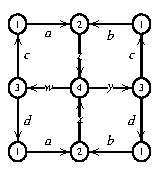
\includegraphics[width=0.22\textwidth]{figures/Fig_241_PDF349_Book337.pdf}
  \caption{习题 11.3 的二聚体模型（原书 p.337）}\label{fig:stability-exercise-dimer-one}
\end{figure}
\begin{enumerate}[label=(\roman*)]
  \item 计算其 Newton 多边形，确定所有完美匹配，并将它们对应到各自格点。
  \item 令 $\alpha=(1,\ldots,1)$。确定满足 $\theta\cdot\alpha=0$ 且使 $M^t_\theta(\mathrm{Jac}\,Q,\alpha)$ 光滑的所有 $\theta$ 所成的集合。
  \item 证明所有光滑的 $M^t_\theta(\mathrm{Jac}\,Q,\alpha)$ 都是同构簇。
\end{enumerate}
\end{exercise}

\begin{exercise}\label{exer:stability-second-dimer}
考虑环面上的下图二聚体模型：
\begin{figure}[H]\centering
  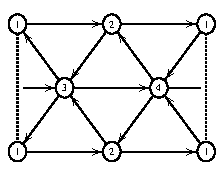
\includegraphics[width=0.37\textwidth]{figures/Fig_242_PDF349_Book337.pdf}
  \caption{习题 11.4 的环面二聚体模型（原书 p.337）}\label{fig:stability-exercise-dimer-two}
\end{figure}
\begin{enumerate}[label=(\roman*)]
  \item 计算其 Newton 多边形，确定所有完美匹配，并将它们对应到各自格点。
  \item 令 $\alpha=(1,\ldots,1)$。确定满足 $\theta\cdot\alpha=0$ 且使 $M^t_\theta(\mathrm{Jac}\,Q,\alpha)$ 光滑的所有 $\theta$ 所成的集合。
  \item 证明所有光滑的 $M^t_\theta(\mathrm{Jac}\,Q,\alpha)$ 都是同构簇。
\end{enumerate}
\end{exercise}

\begin{exercise}\label{exer:stability-tropical-curve}
使用习题\ref{exer:stability-first-dimer} 中的二聚体模型。
\begin{enumerate}[label=(\roman*)]
  \item 找到权函数 $w\colon Q_1\to\mathbb Q$，使相应的特征标为 $\theta=(-3,1,1,1)$。
  \item 确定稳定完美匹配。
  \item 画出相应热带曲线，并在热带曲线上标出二聚体的每条箭。
\end{enumerate}
\end{exercise}

\begin{exercise}\label{exer:stability-linear-quiver-hn}
设 $Q$ 是三顶点线性箭图：
\begin{figure}[H]\centering
  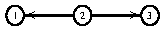
\includegraphics[width=0.24\textwidth]{figures/Fig_243_PDF350_Book338.pdf}
  \caption{习题 11.6 的线性箭图（原书 p.338）}\label{fig:stability-linear-quiver-exercise}
\end{figure}
考虑一种稳定条件，使简单对象的中心荷为
\[
  Z(S_1)=1+i,\qquad Z(S_2)=i,\qquad Z(S_3)=-1+i,
\]
且它们的相位都位于 $(0,\pi)$。考虑 $\mathrm{mod}^{\bullet}Q$ 中所有不可分解对象，并给出它们的 Harder--Narasimhan 滤过。
\end{exercise}

\begin{exercise}\label{exer:stability-unique-acyclic}
证明：若 $A=\mathbb CQ/I$，其中 $Q$ 没有有向环，且
\[
  C\colon Q_0\longrightarrow\{re^{i\phi}\mid r>0,\ 0<\phi<\pi\}
\]
是任意映射，则在 $D\mathrm{mod}^{\bullet}Q$ 上恰有一个 Bridgeland 稳定条件，使每个简单模 $S_v$ 的中心荷为 $C(v)$，且相位位于 $(0,\pi)$。
\end{exercise}

\begin{exercise}\label{exer:stability-polynomial-quadratic-differential}
设 $\varphi=(z^2-1)(dz)^2$ 是 $\mathbb P^1$ 上的二次微分。为以 $\varphi$ 的极点为标记点的曲面构造弧系，并赋予由该二次微分诱导的分次。确定相应的 gentle $A_\infty$ 代数。
\end{exercise}

\begin{exercise}\label{exer:stability-three-parameter-differentials}
设 $Q$ 是下图箭图。
\begin{figure}[H]\centering
  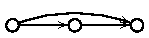
\includegraphics[width=0.23\textwidth]{figures/Fig_244_PDF350_Book338.pdf}
  \caption{习题 11.9 的箭图（原书 p.338）}\label{fig:stability-quiver-exercise}
\end{figure}
\begin{enumerate}[label=(\roman*)]
  \item 给出一个三参数族的 $\mathbb P^1$ 上二次微分，使它们为 $D\mathrm{mod}^{\bullet}Q$ 定义稳定条件。
  \item 画出一个二次微分，使 $Q$ 的所有简单表示具有相同的中心荷和相位。
\end{enumerate}
\end{exercise}

\begin{exercise}\label{exer:stability-chain-p1}
令 $X=\mathbb A^1_0\sqcup_0\mathbb P^1$。确定 $D\mathrm{Coh}^{\bullet}_{\mathbb P^1}X$ 的稳定条件空间。
\end{exercise}

\chapterreview{%
\textbf{全章地位。}本章把稳定性条件从表示论搬到 $A$ 侧与 $B$ 侧：先以格罗滕迪克群给对象分类，再以 King 稳定性造模空间，随后抽象为 Bridgeland 稳定条件，最后用二次微分把它几何化。它承接第 9 章的组合模型与第 10 章的分次版本，并为第 12 章“填充标记点构造闭曲面镜像”提供“特殊曲线即半稳定对象”的直觉。

\textbf{知识脉络。}格罗滕迪克群 $K_0$ 与 Euler 型 $\to$ 箭图表示上以维数向量与参数 $\theta$ 造模空间（King）$\to$ 抽象为扭曲完备 $A_\infty$ 范畴上的二元组 $(Z,\mathcal P)$ 与五条公理（Bridgeland）$\to$ 在分次曲面上用 $\int\omega$（或双覆盖上的 $\int\sqrt\varphi$）作中心荷、用平直度量下的特殊曲线造切片 $\to$ 说明二次微分给出的稳定条件恰好铺满 $\operatorname{Stab}$ 的一个连通分支。每一步都在把依赖具体模型的计算换成范畴内蕴的结构。

\textbf{核心结论。}（1）$K_0\mathrm{topFuk}^{\bullet}(\vec S,M)\cong H_1(\vec S,M)$；Euler 型 $\langle X,Y\rangle=\sum_i(-1)^i\dim A^i(X,Y)$，带对象之间的配对就是交数。（2）King 稳定性：$M_\theta(A,\alpha)=\operatorname{Proj}R_\theta$，$\theta$ 稳定指不存在维数向量 $\beta$ 满足 $\beta\cdot\theta\le0$ 的真子表示，且模空间非空须 $\theta\cdot\alpha=0$。（3）Ishii--Ueda：通有 $\theta$ 下 $Y_\theta=M^t_\theta$ 是匹配多边形所定仿射环簇 $Y$ 的消解，且 $D\mathrm{Coh}^{\bullet}Y_\theta\cong_\infty D\mathrm{Mod}^{\bullet}\mathrm{Jac}(Q)$、$\mathrm{MF}^{\pm}(Y_\theta,\ell)\cong_\infty\mathrm{MF}^{\pm}(\mathrm{Jac}(Q),\ell)$；稳定对给出带对象，热带曲线复原三角剖分。（4）Bridgeland 五条公理推出 Harder--Narasimhan 滤过与心 $\heartsuit_\sigma$，$\operatorname{Stab}_\Gamma A^{\bullet}$ 是复流形，遗忘映射为局部微分同胚。（5）$\mathrm{Flat}(S^{\flat})\to\operatorname{Stab}(S^{\flat})$ 是开闭嵌入，即一个连通分支；Takeda 定理在无内部标记点且某边界分支有两个标记点时给出 $\mathrm{Flat}=\operatorname{Stab}$。

\textbf{辨析与提醒。}其一，相位只在模 $\pi$ 意义下定义（公理 SC2），心取半开区间 $(0,\pi]$，比较相位前必须先固定平移。其二，$\beta\cdot\theta\le0$ 的方向随 $\theta$ 变号而翻转，而“模空间非空 $\Leftrightarrow\theta\cdot\alpha=0$”常被漏掉。其三，$Z(L)$ 可能为无穷（端点落在高阶极点），只有避开极点的子范畴 ${}^{\mathrm{fin}}\mathrm{Fuk}$ 才带稳定条件。其四，“稳定流形”不是“稳定条件空间”的同义词：$\mathrm{Flat}$ 一般只是 $\operatorname{Stab}$ 的一个分支，等号仅在 Takeda 型条件下成立；第 11.5 节的三个例子分别给出 $\mathbb C^n$、$\mathbb C^2$ 与 $\mathbb C\times\mathbb H^+$，恰好说明分支可以很小。

\textbf{评注。}先 King 后 Bridgeland 的次序是有意的：King 可算，二聚体、环簇与热带曲线三件工具都能落地；Bridgeland 抽象，却提供与几何的接口。作者也诚实标出局限：只做曲面，只做 $\mathbb Z_2$ 或分次情形，$\operatorname{Stab}$ 的整体连通性几乎未触及。全章真正的桥是“特殊曲线即半稳定对象”，它把 Harder--Narasimhan 分解读成“把曲线在同伦类里拉直”。若只记住公理而漏掉这条几何图像，第 12 章用变形消去弦端点的构造会显得突兀；反过来，先读第 11.4 节的条带分解，再回头看形变理论，会顺畅得多。日后要处理高维或代数簇上的稳定性，King 与 Bridgeland 两套语言仍需并用，本章的对照正可作模板。}
